\documentclass[shortabstract, english, mgr]{iithesis}
\usepackage[utf8]{inputenc}  
\usepackage{graphicx}    
\usepackage{epstopdf}
\usepackage{amsmath,amsfonts,amsthm,mathtools}
\usepackage{bbm}  
\usepackage{hyperref}
\usepackage{url}
\usepackage{algorithmic}
\usepackage{float}
\usepackage{array}
\usepackage{algorithm}
\usepackage{braket, booktabs}
\setlength\extrarowheight{3pt}

\DeclareMathOperator*{\argmax}{arg\,max}
\DeclareMathOperator*{\argmin}{arg\,min}
\newtheorem{lem}{Lemma}

\usepackage{afterpage}

\newcommand\blankpage{%
    \null
    \thispagestyle{empty}%
    \newpage}
    
\renewcommand{\labelitemi}{\textbullet}

\author{Stanisław Wilczyński}
\englishtitle{Microarray data analysis in prediction of breast cancer metastasis}
\polishtitle{Analiza mikromacierzy DNA w predykcji przerzutów raka piersi}

\englishabstract{One of the major problems of modern medical studies is the prediction of future metastases of breast cancer diagnosed patients. Although metastases are the main cause of death of such subjects and despite the effort in uncovering the underlying mechanism, there was only a minimal improvement in the field in recent years. The mechanism of distinguishing people having high risk of developing a distant metastases from the low risk group could greatly reduce the number of inmates unnecessarily receiving chemotherapy. Data mining seems to be a great candidate for automating the process of such diagnosis as it could allow to predict the outcome of the disease based on hidden, almost impossible to detect correlations or dependencies within the data. One of the most appealing competitors for highly informative data is the level of gene expression collected from the tumor cells. Unfortunately, the analysis of gene expression can be problematic, due to the number of features (measurements of expressed genes) being much higher than the number of samples (patients). In this thesis, we focus on comparing different classification, dimensionality reduction methods in order to find the ones applicable in the field of prediction of future metastases of breast cancer diagnosed subjects and showing that these techniques could help in providing automatic diagnosis and deciding about potential highly toxic treatment.}
\polishabstract{Jednym z głównych celów innowacyjnych badań medycznych jest przewidywanie przerzutów u chorych na raka piersi. Pomimo tego, że przerzuty są jedną z najczęstszych przyczyn śmierci takich pacjentów oraz znacznych nakładów na analizę czynników je wywołujących, tylko niewielki postęp został poczyniony w  tym obszarze w ostatnich latach. Mechanizm pozwalający rozróżnić pacjentów z grupy wysokiego ryzyka pozwoliłby znacznie zredukować liczbę chorych, którzy niepotrzebnie zostają poddani chemioterapii. Metody eksploracji danych wydają się świetnym kandydatem do procesu automatyzacji takiej diagnozy ze względu na możliwość uwzględnienia niewidocznych dla człowieka korelacji między czynnikami wpływającymi na rozwój choroby. Jednym z najbardziej popularnych rodzajów danych służących do tego typu badań są dane poziomu ekspresji genów, pobrane z komurek rakowych. Niestety, taka analiza może być problematyczna ze względu na liczbę próbek (pacjentów) będącą znacznie mniejszą niż liczba zmiennych (poziomy ekspesji różnych genów). W tej pracy skupiamy się na porównaniu różnych metod klasyfikacji oraz redukcji wymiarowości, w celu znalezienia tych najlepiej radzących sobie z przypisywaniem pacjentów do odpowiednich grup ryzyka i pokazaniu, że mogą one pomóc w stworzeniu automatycznego narzędzia diagnostycznego decydującego o przypisaniu chorego na toksyczną terapię.}
\advisor{dr Jan Chorowski}


\begin{document}

\chapter{Introduction}

\section{Overview}
One of the major problems of modern medical studies is the prediction of future metastases of breast cancer diagnosed patients. Although metastases are the main cause of death of such subjects and despite the effort in uncovering the underlying mechanism, there was only a minimal improvement in the field in recent years. The main concern is the lack of reliable method to classify inmates to 'poor prognosis' and 'good prognosis' groups. The first one refers to patients that would develop a distant metastasis within five years since first tumor appearance. According to \cite{Metastasis1} the mechanism of distinguishing between these two classes could greatly reduce the number of subjects unnecessarily receiving chemotherapy. Data mining seems to be a great candidate for automating the process of such diagnosis as it could allow to predict the outcome of the disease based on hidden, almost impossible to detect correlations or dependencies within the data. One of the most appealing competitors for highly informative data is the level of gene expression collected from the tumor cells. There are numerous examples of such data proving to be useful in tumor classification (\cite{BreastCancerClassification}, \cite{TumorMolecularClass}, \cite{TumorsClass1}, \cite{TumorClass2}). Unfortunately, the analysis of gene expression can be problematic, due to the number of features (measurements of expressed genes) being much higher than the number of samples (patients), as the extraction of gene expression data is costly. Such relation causes a phenomenon called 'curse of dimensionality' (\cite[p. 22-26]{ESL2}). In order to decrease this effect the dimensionality reduction techniques are often applied (\cite{MasterArts}, \cite{TumorClass4}, \cite{TumorPLS}). Such reduction even allows to use with success one of the most popular and state-of-the-art techniques such as neural networks (\cite{fDNN}), which do not work in the settings where number of features is significantly higher than number of samples. Another important techniques are building a sparse representation (\cite{TumorClass3}) or using strong regularization (\cite[p. 649-666]{ESL2}) in constructed models. However, in scope of prediction of metastases data-mining methods are not so popular. In fact, current research focus mostly on purely biological markers (\cite{Metastasis4}, \cite{dataOrigin}), use prior knowledge based on protein-protein interaction networks (\cite{MetastasisScores}) or operate on very small samples (less than $100$ patients) and utilize only basic classification methods (\cite{Metastasis1}, \cite{Metastasis2}). Such reluctance to adopt more advanced models is usually caused by the requirement of having a model which can be easy to interpret. In terms of gene expression data it refers to being able to highlight the genes having the highest influence on the response. We use a gene expression data set consisting of $969$ patients for whom $12179$ genes expression levels were measured.

In this thesis we present different classification and dimensionality reduction methods, discuss their advantages and weaknesses and apply them to the gene expression data. The main contribution is showing that these techniques could help in providing automatic diagnosis and deciding about potential highly toxic treatment. The code for all the experiments performed in this thesis is available at \url{github.com/sjwilczynski/geneExpr}.  


In section \ref{section:bio} we explain the medical notions in the simplified form to make it understandable for a person with very little biological knowledge and explain how our data set was collected and processed. In section \ref{section:methods} we discuss the methods used for classification and dimensionality reduction. In section \ref{section:exploratory} we statistically and graphically inspect our data. In section \ref{section:results} we present the results of our analysis and discuss them. In section \ref{section:application} we consider the medical applications and show how specific requirements in the field implies some tuning of our models.

\section{Gene expression data} \label{section:bio}

\subsection{Biological background} 
In this section we briefly explain biological notions used throughout the thesis, based on \cite{NHGRI} and \cite[chapters~11,12]{GeneExpr}. The \textit{cell} is the smallest structural and functional unit of a living organism that is able to run a biological processes (e.g metabolism, growth, reproduction). Every cell contains a \textit{DNA} (deoxyribonucleic acid) which is a chemical compound carrying the information needed to develop and direct the activities of the cell. DNA is composed two chains coiling around each other, which are made of four basic chemical units called nucleotides. A \textit{DNA sequence} is a particular arrangement of these nucleotides within a chain. This arrangement is what codes a unique characteristic of an organism. A \textit{genome} is an entire DNA sequence of a living creature. A \textit{gene} refers to a specific fragment of genome that has a distinct purpose, especially carries instructions for producing a RNA molecule and then a protein. \textit{Proteins} and \textit{RNA molecules} are basic functional molecules in organisms, that among many applications within a cell control chemical reactions, regulate growth and participate in communication in biological pathways. In case of DNA mutation, the information it contains can be corrupted, causing a production of undesirable protein and disruption of standard flow of biological process. Such disruption, if undetected by immunological system can lead to diseases development.

\textit{Gene expression} is the process during which the instructions coded in gene are used to synthesize its products. The level of expression corresponds to the amount of molecules created during this process. The gene is \textit{upregulated} if it synthesizes more, and \textit{downregulated} if synthesizes less when compared with such production in some reference conditions, assumed to be a homeostasis. The state-of-the-art technique for measuring relative expression levels is gene expression profiling using DNA microarrays. The main application of microarrays is to discover how genes functioning changes in response to genetic and environmental variations. \textit{Microarray} is a glass or plastic surface with microscopic spots, placed in regular intervals. Each spot contains picomoles ($10^{-12}$ moles) of a specific DNA sequence, known as \textit{probes}, which interact with tested and reference gene expression product, resulting in emitting measurable signal. By using products from two different cells (e.g cancer and healthy) on the same microarray we can measure the ratio of expression. These ratios are later gathered to form a vector of expression ratios of different genes. In order to conduct a research aimed at specific disease we collect vectors for different individuals with common condition and form a matrix. This matrix is referred as \textit{gene expression data}. As stated in \cite{preprocessing} there are two main sources of variations in microarray measurements. The first one called \textit{interesting variation} corresponds to the case when, for example, highly upregulated gene causes an illness and there is a noticeable difference between diseased and normal tissue. However, the other one called \textit{obscured variation} is induced by differences in the process of sample preparation, microarray manufacturing or even collecting the results from an array. Due to such diversity of possible factors influencing the results obtained from a microaaray it is crucial to apply normalization methods before actual data analysis in order to avoid misleading or even completely incorrect conclusions.

A tumor is a mass formed by a group of abnormal cells. This abnormality refer to disruption in the process of division and apoptosis. However, not all tumors are cancerous. The cancerous tumors (referred as malignant) are characterized by uncontrolled growth and division that leads to damaging nearby tissues. The process of spreading cancerous cell from primary source to other parts of body is called metastasis. Simplifying, it can be described as partial detachment of the tumor and its transport with blood to other part of the organism. Such secondary pathological sites are called metastases and are particularly dangerous. The gene expression data is of great interest in cancer related research as the alteration of cancerous cell division pattern is usually caused by either a mutation in a set of genes or a change in expression level.

\subsection{Data description}

The data set consists of $969$ patients. Each patient is represented by the array measurement of the expression level from his cancerous cell. Such measurement has its unique identifier (e.g \textit{GSM177885}) referring to Gene Expression Omnibus (\cite{GEO}, \cite{NCBI2}). Gene Expression Omnibus is public database storing various forms of high-throughput functional genomic data. The repository is maintained by US organization National Center for Biotechnology Information and the data is uploaded and reviewed by scientific community. The \textit{GSM} prefix indicates that this identifiers corresponds to a single sample/cell. Other prefixes refer to series of data gathered within the same conditions (\textit{GSE}), platform (specific micorarray technology) used to perform the experiment (\textit{GPL}), collections of samples assembled by GEO staff (\textit{GDS}). In case of our data set, it was assembled from 10 public microarray data sets, namely: GSE25066, GSE20685, GSE19615, GSE17907, GSE16446, GSE17705, GSE2603, GSE11121, GSE7390, GSE6532. Each series was obtained using Affymetrix Human Genome HG-U133 Plus 2.0 and HG-U133A arrays, which are the types of the mentioned earlier platforms. As explained in \ref{section:bio} it is essential to preprocess data before the analysis. Therefore, each data set was first normalized using quantile normalization described in \cite{quantileNorm}, then further processed using robust multi-array average (RMA) probe summary algorithm from \cite{preprocessing}. Due to the fact that these series could have different number of genes expression measured they were combined together on the basis of HG-U133A array probe names resulting in reducing the number of variables to $12179$. Each variable correspond to a level of expression of a specific gene (e.g. RPL41). Each patient is also labeled. Label $1$ corresponds to people who experienced metastatic event within 5 years from being cancer diagnosed. $0$ corresponds to people who had the first follow up after $5$ years or no metastasis at all. There are $393$ and $576$ samples with labels $1$ and $0$ respectively.

\chapter{High dimensional data analysis} \label{section:methods}

As stated in the introduction our aim is the prediction of future metastases which in terms of our data translates to binary classification problem using the labels. There are numerous examples where classification methods allow to solve very complex problems e.g customer target marketing, document categorization and filtering or computer vision tasks (\cite{dataClassification}). However, in the field of biomedical data not all of them are applicable. The reason is the high dimensional, complex structure of our data, particularly the relation between the number of samples and number of features: $n \ll p$. Such relation is caused by the relatively low availability of samples and high costs of extracting, processing and labeling new ones. These activities have to be done in laboratory by professionals, in comparison to creation of data sets containing images where anyone can participate in e.g paid labelling procedure. Apart from that huge number of features causes a phenomenon called \textit{curse of dimensionality}. As described in \cite[chapter 6.4.3]{ISL} the increase in the number of variables can improve the model only if the added features are signals, i.e. associated with the response. On the other hand, if they do not influence the response at all, they introduce noise. This may lead to overfitting (high variance) and significantly larger test error. The source of this problem is that with increasing dimension the sample space becomes very sparse and all pairwise distances between data points are alike. Furthermore, huge number of variables introduces more complexity in most models as the number of parameters to estimate grows. In extreme cases it may even lead to lack of convergence in parameter estimation procedure and in consequence lack of model stability. In order to tackle this issue we will use robust classifiers and dimensionality reduction methods described in further chapters.

\section{Model assessment and selection} \label{section:selection}

Before introduction of dimensionality reduction and classification techniques we focus on showing how to choose from a variety of different models and how to assess them. These two tasks are quite different and there exists a variety of methods with distinct tradeoffs. Model assessment typically refers to estimation of generalization performance of the model - its predictive power on new, unseen data. In scope of model selection we can distinguish two task. The first one, subtask of the other, is choice of model \textit{hyperparamters} - parameters of the model which are not estimated during training phase but rather provided as an input. An example is a $k$ in k-Nearest-Neighbour classifier or any regularization constant (e.g section \ref{section:logit}). The other one is the choice of learning algorithm - not only we want to find the best parameters but also be able to determine which classifier is best-suited for our problem. One key difference between model assessment and selection is that in case of the latter we only need to measure relative performance of the models - they may be biased on condition that bias influences all models equally. In case of model assessment we are only interested in unbiased estimators of generalization performance.

In order to further elaborate on evaluation techniques we introduce two key notions: model \textit{bias} and \textit{variance}. Bias refers to the magnitude of difference between model's mean prediction and mean true value. Big bias indicates that our model is not able to take into account most of the dependencies within our data set - it hints that our model is either too simple for the data or its assumptions are not held (undefitting). Variance is a measure of model's prediction instability. Big variance suggests that our model is very sensitive to small perturbations in the data set - it indicates that our model is too complex to our data and has too many degrees of freedom (overfitting). These two values are usually complementary. To see this, consider a model assessment task. We cannot estimate generalization performance using the data set used for fitting the model, as on this set we can only measure the bias that tends to decrease with model complexity. However, large variance may cause the model to perform poorly on new data. Therefore, we split our data to two parts train set and test set. On the train set we fit the model and on the test set we check its prediction performance. As the latter set was not used during fitting process, if the set was split in reasonable manner, the prediction accuracy on the test set is a good estimate of the generalization performance. Such split allows us to capture the crucial statistical phenomenon, i.e \textit{bias-variance tradeoff} (figure \ref{fig:biasVarTrade}). 

\begin{figure}
\centering
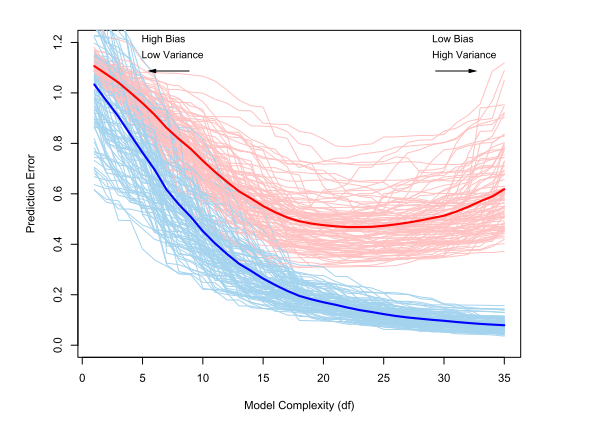
\includegraphics[width=\textwidth]{images/BiasVarianceTrade.png}
\caption{Bias variance tradeoff. The picture comes from \cite{ESL2} - figure 7.1}
\label{fig:biasVarTrade}
\end{figure}

The figure shows in blue prediction error curves on the train set and in red prediction error curves on test set for 100 different splits. The solid curves are the mean curves. On the x axis we have a model complexity. The left side of the plot is region of high bias and low variance - model does not capture dependencies in the data but the predictions are very stable. Then as the model is getting more complex and accurate for the data, the variance and bias together decrease. However, for some model complexity the variance reaches its minimum and starts increasing while bias still decreases. That is where the name of the phenomenon comes from - in order to minimize the prediction error we cannot only use more elaborate models and decrease bias. We need to find a point for which the sum of contributions of errors resulting from bias and variance is minimized. That is our goal in the process of model assessment - choose a model capturing most of the regularities in our data but also with good generalization performance. The question arises of how to fairly split our data set to train and test sets. The fully random approach may result in proportions of classes in both sets to be different from the proportions in the original one. This may result in biased evaluation of model performance. In order to discard this problem we need to use \textit{stratified} sampling - the data is split based on class labels to two groups and the random sampling takes places in both of them to keep the same proportions of classes in train and test sets. The other issue are the sizes of each set. We want a test set to be representative so that it provides good estimation of generalization performance, but we also want to keep the training set as large as possible as the number of data samples needed to properly train the model increases with model complexity.  The typical choices of train/test split are 2/1, 3/2, 3/1, 4/1 but the decision depends on specific problem.  

Nonetheless, train/test split is not enough when we want to tune hyperparameters of the model and estimate its performance on unseen samples. If we used the performance on the training set to select the model, we would choose the one that most overfits on the train data instead of the one that generalizes best. On the other hand, if we use the performance on the test set, it would be positively biased estimate of generalization performance. The reason is although the model did not use test set during learning process, it was used during selection, favouring models performing well on this particular samples from population. Therefore, instead of two-way split we require a three-way split, i.e train/validation/test split. The models learn using only the train set with different values of hyperparamters. Then we compare the performance of these models on the validation set and select the best one. Finally, the generalization performance is estimated using the test set. Again the split should be performed using stratified sampling and typical train/validation/test ratios are: 2/1/1, 3/1/1.

However, two-way split is not the only method for the estimation of the generalization performance and train/validation split is not the only method for model selection. The most popular alternative technique is $k$-fold cross-validation. It tackles the issue of holdout method, i.e not using a big part of data for training and another larger part for testing. We divide the data set in stratified manner to equally sized $k$ folds. In the $i$-th iteration we evaluate the model, trained using all folds but $i$-th, on $i$-th fold used as a test set. After $k$ iterations we have $k$ estimates of the generalization performance and we use their mean as the final estimate. If we use cross-validation for model selection we do the above steps for each choice of hyperparameters and use the mean performance on test folds as the selection metric. The important properties of cross-validation are:
\begin{itemize}
    \item Instead of providing single estimate of generalization performance it gives $k$ values - we can use them not only to compute mean estimate but also standard deviation in order to see how stable is our estimate.
    \item Each data point is used both in training and in test/validation phase but never in both simultaneously - this is particularly important for small data sets when we do not want to introduce pessimistic bias resulting from too few samples used for model training.
    \item Is is much more computationally demanding then train/test split method - it fits $k$ model instead of one.
\end{itemize}
The last point is the reason why cross-validation is rarely seen in deep learning problems - training a neural net is usually too costly to be performed that many times especially for hyperparameter tuning. Also the data sets are often large enough to be able to holdout a validation and test parts without risking that too few samples will be used in learning phase to train the model properly. Cross-validation has one more issue - how to choose $k$. As stated in \cite{ModelSelection} with increasing $k$ the bias of performance estimator decreases but variance and computation cost grow. On the other hand, for small data sets small values of $k$ result in higher variance because of the effect of random sampling. Therefore, typical choice for very limited data sets is $n$, where $n$ is the number of samples. In other cases, $4,5,10$ are most commonly used.  

So far we discussed model assessment and model selection in terms of hyperparameter tuning. However, the most interesting issue in our study is the selection of algorithm together with hyperparamters. As it turns out we cannot use standard cross validation for this task as it usually results in biased results (\cite{ModelSelection}, \cite{cvOverfit}). Therefore, we use \textit{nested cross-validation} introduced in \cite{nestedCV}. It is presented graphically in figure \ref{fig:nestedCV}.

\begin{figure}
\centering
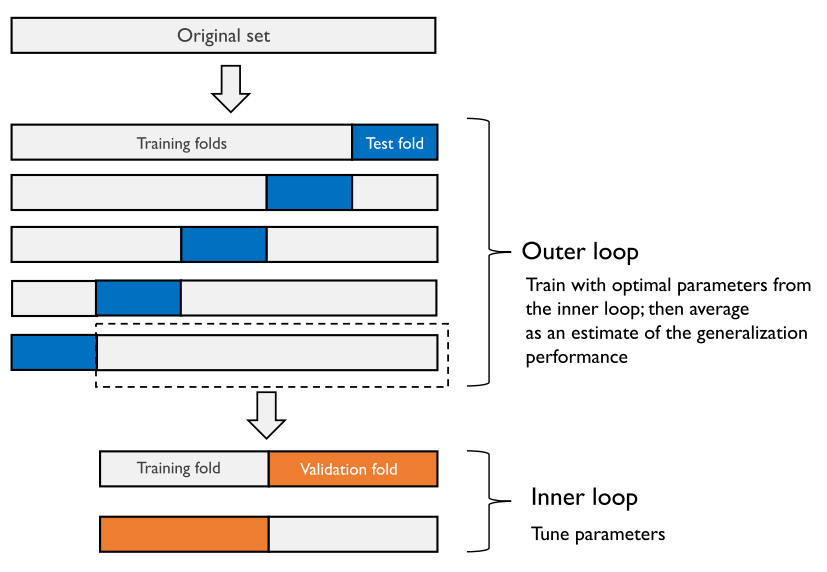
\includegraphics[width=\textwidth]{images/nestedCV.png}
\caption{Nested cross validation - picture comes from \cite{ModelSelection}, figure 22}
\label{fig:nestedCV}
\end{figure}

The main idea is a usage of two nested cross-validation loops. In the inner loop we tune model hyperparameters and in the outer loop we estimate its performance in order to compare fairly different learning algorithms. For our particular task we would use 5x2 setup (5 folds in outer loop, 2 in the inner one). As we use this technique for selection among different methods we still keep the holdout test set to later assess the performance of the chosen approach.

Although we presented a few model selection and assessment techniques we still have to refer to performance metrics as they are key part of this process. The simplest one is the accuracy - percentage of correctly classified samples among the data. However this metric is not perfect, particularly in cases of imbalanced classes. Imagine an artificial binary classification problem where one of the classes is represented only by $10\%$ of the data. Then a classifier that always assigns the other label has $90\%$ accuracy - quite high for a model that does not capture any regularities in our data and is completely useless. Therefore, we use more reliable metrics for both model comparison and generalization performance estimation. Let us assume that we have a trained model and a data set on which we want to evaluate it. Let us introduce four factors:
\begin{itemize}
    \item True positives (TP) - number of samples that are from class $1$ and model predicted $1$.
    \item False positives (FP) - number of samples that are from class $0$ but model predicted $1$.
    \item False negatives (FN) - number of samples that are from class $1$ but model predicted $0$.
    \item True negatives (TN) - number of samples that are from class $0$ and model predicted $0$. 
\end{itemize}
In case of our data set class $1$ correspond to patients experiencing metastatic event within 5 years from first diagnosis. Using these four values we can define three classification metrics:
\begin{itemize}
    \item Precision- $\frac{TP}{TP + FP}$
    \item Recall (or true positive rate (TPR), sensitivity) - $\frac{TP}{TP + FN}$
    \item F1-score - harmonic mean of precision and recall
\end{itemize}
By using our case as an example precision measures how many patients that are assigned to class $1$ really experienced a metastatic event. On the other hand, recall measures how many of the patients who experienced a metastatic event actually are assigned to class $1$. In complex classification problems there is tradeoff between these two metrics - optimizing one of them results in decrease in the other. However, in our case we are more interested in having high recall - as the error of not assigning the patient to high risk group and in consequence not applying a therapy in a case he is to experience a metastatic event is much more harmful than applying treatment for patient of low risk. The first error may result even in patient's death. Still, for model selection it is crucial to have a metric that we can use for direct comparison. One of the potential choices is F1-score, combining both precsion and recall in one measure, but in our study we use area under the curve (AUC) of receiver operating characteristic curve (ROC). ROC curve is the name for the plot of TPR against False Positive Rate (FPR, $\frac{FP}{FP + TN}$). Using the AUC we can measure how good is our model at separating positive from negative class and also find a good threshold for decision boundary (by default if our model returns probabilities it is 0.5). To draw the ROC curve we need to rank our samples decreasingly by classifier score (assuming that higher score refers to greater certainty of positive class). We start at point $(0,0)$ and assume that we have $pos$ samples labeled as $1$ and $neg$ samples labeled as $neg$. Starting from the top of the ranking if the label is $1$ we move up by $\frac{1}{pos}$ and if the label is $0$ we move by $\frac{1}{neg}$ right. To visualize this on figure \ref{fig:roc} we present two example curves - the one on the right is the curve for the perfect classifier and the one on the left is a curve for more an artificial classification problem modeled using logistic regression.

\begin{figure}
\centering
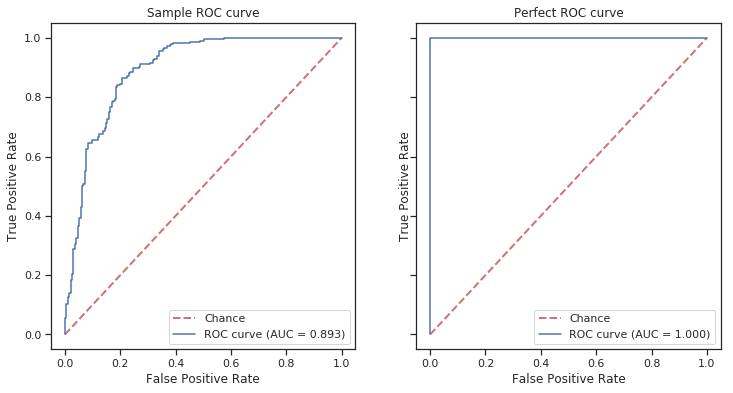
\includegraphics[width=\textwidth]{images/rocExample.png}
\caption{Example ROC curves}
\label{fig:roc}
\end{figure}

If we used a random classifier for balanced classes we would obtain a ROC curve equal to $x=y$ line. Therefore this line is treated as baseline and is present in the plots. The AUC for the perfect classifier is $1$ and for the baseline is $0.5$. The AUC may be interpreted as expectation that uniformly drawn positive sample is ranked before a uniformly drawn negative sample. As mentioned before in our problem we care much more about high TPR than low FPR, therefore we would exploit the features of ROC and we will adjust decision threshold values.

\section{Classifiers for high dimensional data}

\subsection{Logistic regression and its modifications} \label{section:logit}

One of the most popular and simple classifiers for binary response is logistic regression (LR). It is a counterpart of linear regression for regression problems and was proven to be valuable method for microarray analysis (\cite{LRgene}). The model aims at estimating the conditional probability of class membership. It is described by the following formula:
\begin{align*}
    &P(y=1 | x, \beta)=\sigma\left(\beta^{T} x\right) \\
    &\sigma(t) = \frac{1}{1+e^{-t}} \\
    &x=(1, x_1, \ldots, x_p)^T \\
    &\beta = (\beta_0, \ldots, \beta_p)^T
\end{align*}
where $x$ is the vector of features with additional $1$ as first coordinate to abbreviate the notation, $\beta$ is the vector of coefficients including intercept, $\sigma$ is sigmoid function and is used to squeeze the output to range $(0,1)$ and P is the conditional probability of class $1$ of a sample described by variables $x$. The interpretation of logistic regression coefficients is quite different from linear regression due to the usage of sigmoid function. In terms of the latter an increase of one unit of variable $x_i$ corresponds to increase of the output by $\beta_i$. The similar relation for LR can be expressed using log odds (the ratio of probabilities of event occurring and not occurring):

\begin{align*}
    \log \left(\frac{P(y=1| x, \beta)}{1-P(y=1| x, \beta)}\right)=\log \left(\frac{P(y=1| x, \beta)}{P(y=0| x, \beta)}\right)=\beta_{0}+\beta_{1} x_{1}+\ldots+\beta_{p} x_{p}
\end{align*}

Above equation clearly indicates that an increase of one unit of variable $x_i$ corresponds to increase of the log odds by $\beta_i$ and this implies and increase of odds ratio by a factor of $\exp(\beta_i)$. Similarly $\beta_0$ corresponds to the log odds in the baseline conditions. Such relatively simple and probabilistic interpretation made the model very popular. However, it has some disadvantages. First of all, it does not incorporate a possibly complicated correlation structure or interactions between variables. Secondly, it could perform worse with highly correlated features or features having no influence on response and coefficients could be infinite in case of complete separation, i.e when one feature can distinguish completely between classes. Nonetheless, LR is widely used, also due to uncomplicated learning scheme. Similarly to linear regression coefficients in LR are calculated using maximum likelihood estimation. The likelihood function takes the form:
\begin{align*}
    L(\beta) &= \prod_{i=1}^n P(Y=y_i | x_i, \beta) \\&= \prod_{i=1}^n P(Y=1 | x_i ; \beta)^{y_i}(1-P(Y=1 | x_i ; \beta))^{\left(1-y_i\right)} \\
&= \prod_{i=1}^n \sigma\left(\beta^{T} x_i\right)^{y_i}\left(1-\sigma\left(\beta^{T} x_i\right)\right)^{\left(1-y_i\right)}
\end{align*}
And the negative log likelihood is:
\begin{align*}
    nll(\beta)=-\sum_{i=1}^{n} y_i \log \sigma\left(\beta^{T} x_i\right)+\left(1-y_i\right) \log \left(1-\sigma\left(\beta^{T} x_i\right)\right)
\end{align*}

In the two above equations $x_1, \ldots x_n$ denote samples and $y_i$ corresponding labels. In order to maximize the coefficients we calculate the first derivative of the negative log likelihood function as in \cite[chapter 4.4.1]{ESL2}:
\begin{align*}
    \frac{\partial nll(\beta)}{\partial \beta}&=\sum_{i=1}^{n}\left(\sigma\left(\beta^{T} x_i\right)-y_i\right) x_i\\ &=
    \left[\left(\sigma(X\beta) - Y\right)^TX\right]^T
\end{align*}
We can clearly see that the right side is not linear in $\beta$ and in fact equation $\frac{\partial nll(\beta)}{\partial \beta} = 0$ cannot be solved analytically. Therefore, the maximizing coefficients are found using Newton-Raphson method, extensions of gradient descent like SAG (\cite{sag}) or SAGA (\cite{saga}) and other e.g. Liblinear (\cite{liblinear}). 

However, classic logistic regression has one more drawback. The maximization of likelihood function usually provides good (in terms of model usability) estimates of the model parameters. However such estimation may be unstable (model with high variance) when the number of data samples is relatively small. The problem is even more evident when $n < p$. Without any constraints in order to fit $p+1$ coefficients we need at least $p+1$ data points, otherwise there are infinitely many solutions. For our data set $n \ll p$ and LR cannot work in such settings. In order to tackle this problem we consider a more probabilistic (Bayesian) point of view - instead of maximizing the likelihood, we will maximize posterior probability of model parameters:

\begin{align}
    P(\beta| X,Y) &= \frac{P(Y | \beta, X)P(\beta)}{P(Y)} \nonumber \\
    \hat{\beta} = \argmax_{\beta} P(\beta| X,Y) &= \argmax_{\beta} P(Y | \beta, X)P(\beta) \label{eq:post}
\end{align}

The first equation is derived directly from the Bayes rule and we can see that in the equation \ref{eq:post} we can neglect the denominator as it is independent of $\beta$. So the first term on the right side of \ref{eq:post} is the likelihood function and the second is the prior distribution over the values of $\beta$. The maximum likelihood estimation is a special case of maximum a posteriori estimation, i.e. when we assume uniform distribution for model parameters.  Choice of MAP estimates over MLE estimates has a significant effect on our learning scheme. Instead of minimizing the negative log likelihood we minimize the expression:

\begin{align}
    J(\beta) &= - \log P(Y | \beta, X)P(\beta) =  - \log P(Y | \beta, X) - \log P(\beta) \nonumber \\ &= nll(\beta) - \log P(\beta) = nll(\beta) - \sum_{i=0}^p \log P(\beta_i) \label{eq:learnPost}
\end{align}

Of course $\argmax_{\beta} P(\beta| X,Y) = \argmin_{\beta} J(\beta)$. The above equation indicates that the mentioned influence depends only on the choice of prior distribution for model parameters. Two popular alternatives are zero-mean normal distribution and zero-mean Laplace distribution:
\begin{align*}
    \mathcal{N}(0, \sigma^2) &\sim \frac{1}{\sqrt{2 \pi \sigma^{2}}} \exp \left(-\frac{x^{2}}{2 \sigma^{2}}\right) \\
    Lap(0, b) &\sim \frac{1}{2 b} \exp \left(-\frac{|x|}{b}\right)
\end{align*}

Putting these two distributions into \ref{eq:learnPost} gives us following versions of $J$ to minimize:
\begin{align*}
    J_{\mathcal{N}}(\beta) &= nll(\beta) + \sum_{i=0}^p -\log \left(\frac{1}{\sqrt{2 \pi \sigma^{2}}} \right) + \frac{\beta_i^{2}}{2 \sigma^{2}} \\
    J_{L}(\beta) &= nll(\beta) + \sum_{i=0}^p -\log \left(\frac{1}{2 b} \right) + \frac{|\beta_i|}{b}
\end{align*}
We can simplify these equations as constants can be discarded during minimization:
\begin{align*}
    \argmin_{\beta} J_{\mathcal{N}}(\beta) &= nll(\beta) + \frac{1}{2 \sigma^2}\sum_{i=0}^p \beta_i^{2} = nll(\beta) + \frac{1}{2 \sigma^2}\| \beta \|_2^2\\ 
    \argmin_{\beta} J_{L}(\beta) &= nll(\beta) + \frac{1}{b}\sum_{i=0}^p |\beta_i| = nll(\beta) + \frac{1}{b}\| \beta\|_1 
\end{align*}
where $||\cdot||_2, ||\cdot||_1$ denote euclidean ($l_2$) and absolute ($l_1$) norms respectively. As we often want to calibrate the influence of the prior of our parameters we rewrite the above to form: 

\begin{align*}
    \argmin_{\beta} J_{\mathcal{N}}(\beta) &=  nll(\beta) + \frac{\lambda_2}{2}\| \beta \|_2^2\\ 
    \argmin_{\beta} J_{L}(\beta) &= nll(\beta) + \lambda_1\| \beta\|_1 
\end{align*}

as increase in either of $\lambda$ makes the prior distribution more significant. This two schemes are called $L_2$ and $L_1$ regularizations. It is also worth noticing that their common general structure can be written as:

\begin{align}
    \hat{\beta} = \argmin_{\beta} \mathcal{L}(X,y, \beta) + \lambda Pen(\beta) \label{eq:loss+pen}
\end{align}

where the first term is called loss function (in our case negative log likelihood) and the second term is called the penalty, where $\lambda$ is the tuning parameter which controls the magnitude of the effect of regularization.

We can see that these two regularizations aim at pushing the coefficients towards zero in order to reduce overfitting and enhance model generalization capabilities. Especially in case of our data, regularization allow us to use LR when $n \ll p$. Yet these two schemes differ considerably. As described in \cite[chapter 13.3.1]{MLprob} the $l_1$ norm favours sparse models (lots of coefficients equal to $0$) and $l_2$ favours models with lots of coefficients having small (but most of the times nonzero) values. The intuition behind this is visible in the formula for the penalty. Consider and example vector $x = (1, \varepsilon)$ where $0 < \varepsilon < 1$. Then the norms are $\|x\|_{1}=1+\varepsilon,  \|x\|_{2}^{2}=1+\varepsilon^{2}$. Now we check how the norms change when we subtract the vectors $(\delta, 0)$ and $(0, \delta)$:

\begin{align*}
    \|x-(\delta, 0)\|_{1}&=1-\delta+\varepsilon, \ \   \|x-(\delta, 0)\|_{2}^{2}=1-2 \delta+\delta^{2}+\varepsilon^{2} \\ 
    \|x-(0, \delta)\|_{1}&=1-\delta+\varepsilon, \ \  \|x-(0, \delta)\|_{2}^{2}=1-2 \varepsilon \delta+\delta^{2}+\varepsilon^{2}
\end{align*}

We can see regularizing the first, larger coordinate in $l_2$ has results in much more significant decrease in norm than doing so for the smaller one. Therefore, it is not very probable that $L_2$ regularization will truncate any tiny coefficients to $0$ as doing so has almost negligible influence on the norm value. In case of $l_1$ the difference in norms is always the same, regardless the actual value of coefficients. That is why $L_1$ regularization is likely to reduce parameters to $0$ if they have minor effects on the likelihood. 

In terms of linear regression these two methods are called ridge regression and LASSO. There also exists a combination of these two i.e. Elastic Net where the penalty is the linear combination of $L_1$ and $L_2$ regularization. As different models can use such regularization in the further chapters we will refer to them as $L_1, L_2$ and Elastic Net penalties.

\subsection{Regularized Discriminant Analysis and Nearest Shrunken Centroid}

As stated in \cite[chapter 18.2]{ESL2} there are two good classifiers that can be used as baseline in high dimensional setting. The first one is Regularized Discriminant Analysis (RDA), an extension of Linear Discriminant Analysis (LDA) (\cite[chapter 4.3]{ESL2}). The assumption of LDA is that samples from each class come from multivariate normal distribution with the same covariance matrix $\Sigma$. In terms of two classes it can be written as:
\begin{align*}
    x_i \sim \begin{cases}
    \mathcal{N}(\mu_0, \Sigma) \text{  if $y_i=0$} \\
    \mathcal{N}(\mu_1, \Sigma) \text{  if $y_i=1$} \\
    \end{cases}
\end{align*}
where $x_i, y_i$ denote $i$-th sample and label in the data set respectively. Let us denote corresponding densities as $f_0$ and $f_1$. Assuming a prior probabilities of class membership $\pi_0, \pi_1, \pi_0 + \pi_1=1$ one can look at the log ratio of class membership probabilities for sample $x_i$:
\begin{align} 
\log \frac{P(Y=1 | x_i)}{P(Y=0 | x_i)}&=\log \frac{f_1(x)}{f_{0}(x)}+\log \frac{\pi_1}{\pi_{0}} \nonumber \\&=\log \frac{\pi_1}{\pi_{0}}-\frac{1}{2}\left(\mu_1+\mu_{0}\right)^{T} \Sigma^{-1}\left(\mu_1-\mu_{0}\right) + x^{T} \Sigma^{-1}\left(\mu_1-\mu_{0}\right) \nonumber\\ &= \delta_1(x_i) - \delta_0(x_i) \text{, where} \nonumber\\
\delta_{k}(x)&=x^{T} \Sigma^{-1} \mu_{k}-\frac{1}{2} \mu_{k}^{T} \Sigma^{-1} \mu_{k}+\log \pi_{k} \label{eq:dslda}
\end{align}
where $\delta_1, \delta_0$ are discriminant scores for classes $1,0$ respectively. As the values of $\mu_1, \mu_0, \pi_1, \pi_0, \Sigma$ are not known, mean sample estimates, class proportions and sample covariance matrix are used. The assumption of equal covariance matrices is why this method is called $linear$. By looking at the ratio of class membership probabilities we can see that quadratic parts from exponent cancelled out resulting in the decision boundary (set where $P(Y=1 | X=x_i) = P(Y=0 | X=x_i)$) to be linear in $x_i$ - a hyperplane. However, if we assume that the covariance matrices are not equal we get a quadratic decision boundary and a method called Quadratic Discriminant Analysis. However, such formulation results in huge number of parameters as each covariance matrix is of size $p \times p$, which is even a problem in LDA. In order to tackle this issue regularization is introduced to form RDA and the covariance matrix is shrunk towards a diagonal one with $\lambda$ as regularization parameter:
\begin{align*}
    \hat{\Sigma}(\lambda)=\lambda \hat{\Sigma}+(1-\lambda) \alpha I
\end{align*}
In the above equation $\hat{\Sigma}$ is the sample covariance matrix and $\lambda$ is the regularization constant. The value of $\lambda$ is chosen using Ledoit-Wolf lemma (\cite{honey}) and $\alpha$ is the average eigenvalue of $\hat{\Sigma}$.


The other method is Nearest Shrunken Centroid (NSC) classifier, described in \cite{NSC}. It is based on a very simple nearest centroid classifier: we calculate centroid for each class and then assign each sample to a class based on its distances to these centroid, i.e. to the one with the smallest euclidean distance. Such elementary algorithm doesn't work in settings where $n \ll p$, due to the curse of dimensionality as described in the beginning of this chapter. Therefore within class centroids coordinates are shrunken toward overall feature mean, making the assignment to classes dependent only on a small subset of variables. To formalize this intuition let us denote $x_{ji}$ as the value of $i$-th variable in $j$-th sample where $i=1, \ldots, p$ and $j=1,\ldots,n$. We assume there are $K$ classes and subset of sample indices for each class is $C_k$ . Let $\bar{x_i}$ denote $i$-th feature mean and $\bar{x_{ik}}$ denote $i$-th feature mean within class $k$. Then we can write:
\begin{align*}
    \bar{x}_{i k}&=\bar{x}_{i}+m_{k} s_{i} d_{i k} \text{, where} \\
    d_{i k}&=\frac{\bar{x}_{i k}-\bar{x}_{i}}{m_{k} \cdot s_{i}} \\ 
    s_{i}^{2}&=\frac{1}{n-K} \sum_{k=1}^{K} \sum_{j \in C_{k}}\left(x_{i j}-\bar{x}_{i k}\right)^{2} \\
    m_{k}&=\sqrt{1 / n_{k}-1 / n} \\
\end{align*}
The values of $m_k$ and $s_i$ are chosen so that $s_i^2$ is a pooled variance and $m_k$ assures that $m_k \cdot s_i$ is the estimated standard error of $\bar{x}_{i k}-\bar{x}_{i}$. With such formulation $d_{ik}$ is a t-statistic for $i$-th feature comparing $i$-th variable mean with a mean within $k$-th class. The shrinkage is applied to $d_{ik}$ creating shrunken centroids $\bar{x}_{ik}^{\prime}$:
\begin{align*}
    \bar{x}_{i k}^{\prime}&=\bar{x}_{i}+m_{k} s_{i} d_{i k}^{\prime} \text{, where} \\
    d_{i k}^{\prime}&=\operatorname{sign}\left(d_{i k}\right)\left(\left|d_{i k}\right|-\Delta\right)_{+}
\end{align*}

This type of shrinkage is called soft thresholding and is just application of proximal operator used for solving problems with $L_1$ regularization. The advantage here is that with a proper choice of $\Delta$ parameter most of the coordinates of class centroid are equal to the coordinates of the whole data set centroid, leaving only few coordinates of each $\bar{x}_{i k}^{\prime} - \bar{x}_{i}$ nonzero. Those few values will be the ones determining the assignment to classes. In terms of our data it translates to making prediction of metastasis dependent only on few chosen genes. It is very reasonable as in microarray analysis most genes does not differ significantly by expression levels between classes and the variability usually comes from random fluctuation and these method aims at removing the noisy features.

With a new sample $x^{*}=\left(x_{1}^{*}, x_{2}^{*}, \ldots, x_{p}^{*}\right)$ to classify we choose the class $k$ with the lowest discriminant score, i.e:
\begin{align}
\delta_{k}\left(x^{*}\right)=\sum_{i=1}^{p}\frac{\left(x_{i}^{*}-\overline{x}_{ik}^{\prime}\right)^{2}}{s_{i}^{2}}-2 \log \pi_{k} \label{eq:dsnsc}
\end{align}

The first part of this score corresponds to the normalized distance to shrunken centroid and the second one results from a simple prior distribution put on class assignment where $\pi_{k} = \frac{|C_k|}{n}$. By expanding the square in equation \ref{eq:dsnsc} we could see that discriminant score in NSC is very similar to discriminant score for LDA (as in equation \ref{eq:dslda}). In fact the distinctions are that NSC assumes diagonal covariance matrix and uses shrunken centroids instead of sample means. The first one is particularly useful in high dimensional data as covariance matrix is of size $p \times p$ and may influence the stability of scores calculations and therefore usability of the model.

\subsection{Linear Support Vector Classifier}

Support Vector Classifier (SVC, \cite[chapter 9]{ISL}) is one of the best "out of the box" classifiers, known to be effective in high dimensional spaces. The technique is based on the concept of maximal margin classifier. Let us denote a data set $X_{n \times p}$ consisting of $n$ samples and $p$ features and a set of labels $Y = (y_1, \ldots, y_n)$ and for simpler classifier rule formulation instead of $y_i \in \{0,1\}$ we have $y_i \in \{-1, 1\}$. We assume our data is completely separable by a hyperplane and our aim is to find it. Such hyperplane can be described by equation:
\begin{align*}
    \beta^T x + \beta_0 = 0 \text{ ,where $\beta = (\beta_1, \ldots, \beta_p)$}
\end{align*}
Without loss of generality we can assume that samples with label $1$ are the ones above the separating hyperplane. In such case the hyperplane has following property:
\begin{align*}
    y_i(\beta^T x + \beta_0) > 0, \ \forall_{i=1, \ldots, n}
\end{align*}

Such characteristic can be exploited to construct very simple classifier: assign new sample $x^*$ to class $1$ if $\beta^T x^* + \beta_0 > 0$ and to $-1$ if $\beta^T x^* + \beta_0 < 0$. Notice that the magnitude of $|\beta^T x^* + \beta_0|$ determines how far is the sample from our hyperplane and in consequence how confident we are about the assignment. Of course if the data is indeed completely separable there are infinitely many separating hyperplanes. However, we choose the maximum margin hyperplane, i.e the hyperplane that maximizes the distance to the closest point to the hyperplane and additionally our minimal confidence about sample assignment within the data. That distance to closest point is called the margin and the points that are exactly margin away from the hyperplane are called support vectors. The intuition for such naming is that even slight change of any of these points changes the hyperplane. Whereas for all other samples the hyperplane is independent, i.e if they are perturbed they do not effect the hyperplane unless they are within margin distance from the separating hyperplane. The 2D example of few possible hyperplanes and the optimal one can be found on figure \ref{fig:svc-hyper}.

\begin{figure}
\centering
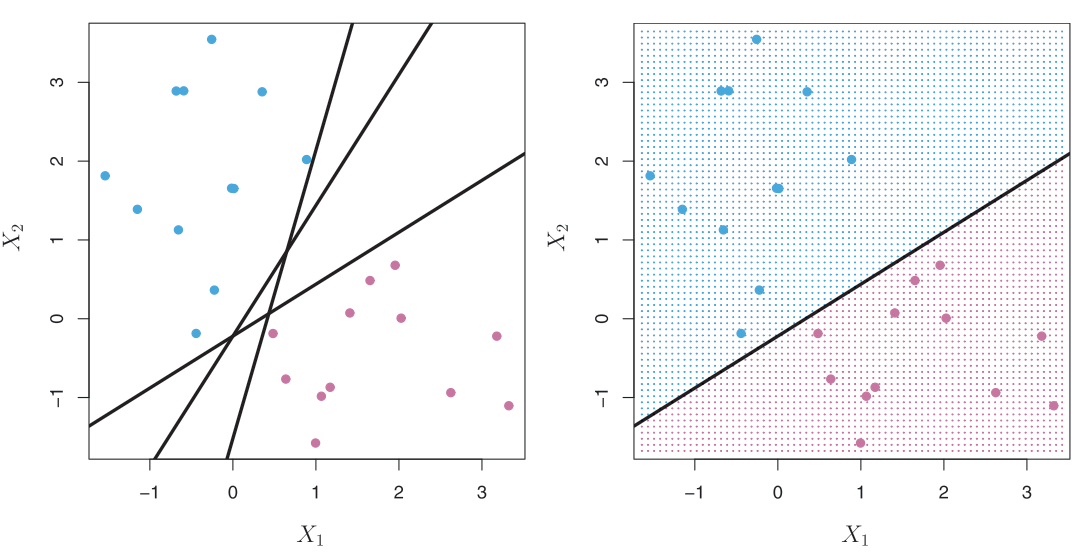
\includegraphics[width=\textwidth]{images/svc-hyper.png}
\caption{Example hyperplances in 2D case. The picture comes from \cite{ISL} - figure 9.2}
\label{fig:svc-hyper}
\end{figure}

To formalize the problem of finding the maximum margin hyperplane we can write:

\begin{align*}
&{\argmax_{\beta_{0}, \beta} \ M} \\ &{\text { subject to } \|\beta\|_2^2 = 1}, \\ &{y_{i}\left(\beta_{0}+\beta^T x_i\right) \geq M \ \forall_{i=1, \ldots, n}}
\end{align*}

The inequality represents the condition that each point has to be at least by $M$ far from boundary, the norm constraint is used for uniqueness as $\beta_0 +\beta^Tx = 0$ represents the same subspace as $k\cdot(\beta_0 +\beta^Tx) = 0$. Also it ensures that the perpendicular distance from $x_i$ to hyperplane is equal to $y_i\left(\beta_0 + \beta^Tx_i\right)$. So $M$ is in fact the exact margin. This optimization problem can be rewritten to get rid of $M$. The inequality condition can be replaced by $y_{i}\left(\beta_{0}+\beta^T x_i\right) \geq M\|\beta\|$ and thanks to the solution being invariant to scaling $\beta$ by a constant we can arbitrarily set $\|\beta\| = \frac{1}{M}$. In such case the problem can be formulated discarding $M$:

\begin{align*}
& \argmin_{\beta, \beta_0} \frac{1}{2}\|\beta\|^2_2 \\ &{\text { subject to }} {y_{i}\left(\beta_{0}+\beta^T x_i\right) \geq 1 \ \forall_{i=1, \ldots, n}}
\end{align*}

The above is convex optimization problem and can be solved using Lagrange multipliers. However, in real world examples data is usually not linearly separable. SVC tackles this issue by finding a hyperplane that nearly separates all samples using \textit{soft margin}. Another advantage is that even in case of separable data finding not necessarily perfect hyperplane allows the model to perform better on unseen data. At the figure \ref{fig:svc-robust} we can see that adding a single sample to our data may change the hyperplane dramatically - possibly decreasing efficiency when classifying unseen data due to very narrow margin. 

\begin{figure}
\centering
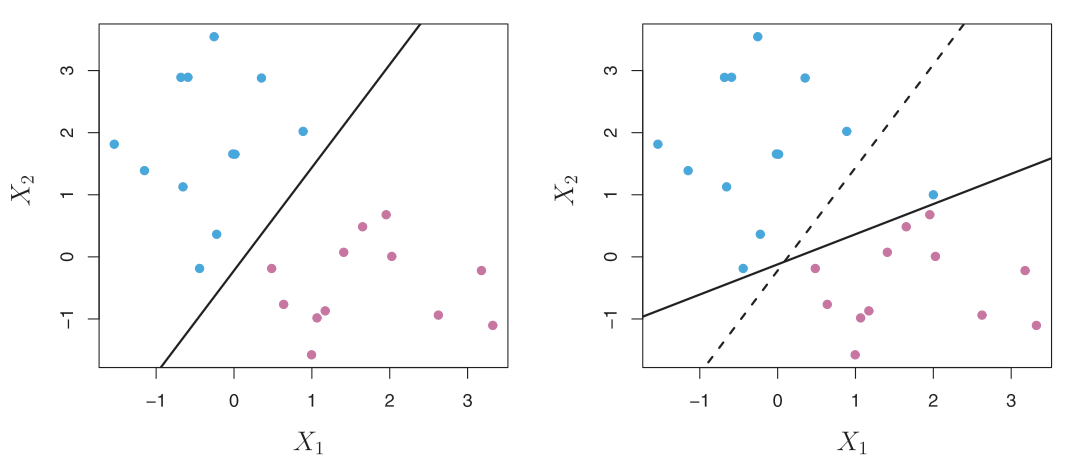
\includegraphics[width=\textwidth]{images/svc-robust.png}
\caption{Changes of maximum margin hyperplane when added one data point. The picture comes from \cite{ISL} - figure 9.5}
\label{fig:svc-robust}
\end{figure}

The another issue is the decrease of confidence of our assignment for many samples near the margin. Therefore, we change our aim from perfect separation to greater confidence about most samples, ensuring robustness to individual points. We allow few data points to be on the wrong side of the hyperplane for the cost of penalty, which increases with the distance from the correct subspace. Using the formula it can be written as:

\begin{align*}
&{\argmax_{\beta_{0}, \beta} \ M} \\ &{\text { subject to } \|\beta\|_2^2 = 1}, \\ &y_{i}\left(\beta_{0}+\beta^T x_i\right) \geq M(1 - \epsilon_i), \\
& \epsilon_i \geq 0, \ \sum_{i=1}^n \epsilon_i < C \ \forall_{i=1, \ldots, n}
\end{align*}

Again we can discard $M$ by reformulating the problem to:
\begin{align*}
& \argmin_{\beta, \beta_0} \frac{1}{2}\|\beta\|^2_2 \\ &{\text { subject to }} y_{i}\left(\beta_{0}+\beta^T x_i\right) \geq 1 - \epsilon_i, \\ &\epsilon_i \geq 0, \ \sum_{i=1}^n \epsilon_i < C \ \forall_{i=1, \ldots, n}
\end{align*}

For computational convenience the above can be presented in equivalent form:
\begin{align}
& \argmin_{\beta, \beta_0} \frac{1}{2}\|\beta\|^2_2 + C \sum_{i=1}^n \epsilon_i \nonumber \\ &{\text { subject to }}\epsilon_i \geq 0, \ \  y_{i}\left(\beta_{0}+\beta^T x_i\right) \geq 1 - \epsilon_i, \ \forall_{i=1, \ldots, n} \label{eq:svcform1}
\end{align}
C is the hyperparameter determining how strong we penalize samples being on the wrong side of the margin. In case of $C = \infty$ SVC is equivalent to maximum margin classifier. On the other hand, small values of C result in allowing more points to be on the wrong side of the hyperplane. The $\epsilon_i$ are known as slack variables. The value of each $\epsilon_i$ determines the relative position to hyperplane. $\epsilon_i=0$ indicates that $x_i$ is on the correct side of hyperplane, at least margin away from it. $0< \epsilon < 1$ means that $x_i$ is on the correct side but within margin distance from subspace. Finally, $\epsilon > 1$ means that $x_i$ is on the wrong side. The notion of support vectors also gets extended to include points not only exactly on the margin but also the ones for which $\epsilon_i > 0$. The classification rule remains the same as for maximum margin classifier. Therefore, the decision on class assignment of new samples is based only on support vectors, i.e. potentially small subset of observations. This characteristic contrasts logistic regression and RDA as their decision rule always depend on all observations. However, some similarities to the first method can be shown. The condition in equation \ref{eq:svcform1} is equivalent to $\forall_{i=1, \ldots, n} \epsilon_i \geq \max \left(0, 1 - y_i(\beta_0 + \beta^Tx_i) \right)$. If we minimize the target that includes sum of $\epsilon_i$ then all inequalities will have to be equalities. Additionally denoting $\lambda := \frac{1}{C}$ we can write the equivalent form of our minimization problem:
\begin{align*}
    \argmin_{\beta_0, \beta} \sum_{i=1}^n \max \left(0, 1 - y_i(\beta_0 + \beta^Tx_i)\right) + \frac{\lambda}{2} \|\beta\|^2
\end{align*}
which is as in case of regularized logistic regression: a loss term + $L_2$ penalty term. This loss is called \textit{hinge loss} and it behaves similarly to negative log likelihood loss in LR, as for the points far from decision boundary the latter gives very small values.

\subsection{Ensemble learning}

In this section we describe two classification techniques based on the concept of ensemble learning. Ensemble learning is a method of training multiple models and aggregating their results to produce a prediction for a sample. These models may be very simple and poor classifiers by themselves but a group of them may form a powerful predictor. The first of these techniques is Random Forest introduced in \cite{RF}. Here the simple learners are decision trees. Decision tree splits the feature space to a number of regions using feature value based rules and assigns a new sample to a class which is a majority in the resulting region for this data point. An example of classification decision tree can be seen on figure \ref{fig:decision-tree}.

\begin{figure}
\centering
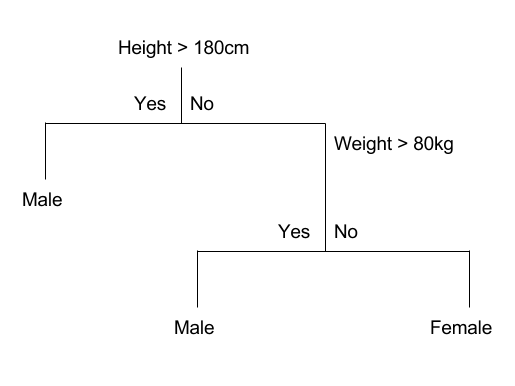
\includegraphics[width=0.7\textwidth]{images/decision_tree.png}
\caption{An example of a decision tree from \url{https://machinelearningmastery.com/classification-and-regression-trees-for-machine-learning/}}
\label{fig:decision-tree}
\end{figure}

This tree has two internal nodes. The decision rule in the upper one, i.e root splits the data to two subtress based on \textit{height} threshold, which is $180$cm. The left node is not further split. In the right subtree we split the data again based on weight and two resulting nodes are also leaves. The label in the leaf indicates which class stands for the majority of training data in the corresponding region. For a new sample we traverse the tree from the root following the decisions in the nodes and assign it to a class that is label of the leaf to which it falls. In general case, in the root of the tree we have one of our variables and some threshold - the data is then split according to the threshold to left part and right part of the tree. In each subtree either the process continues, a variable and a threshold are chosen and part of the data is split again or the splitting stops and the node remains the leaf of the tree representing one of regions in the feature space. As the rules are simple thresholds all the resulting segments are hyperrectangles. In order to learn such tree we have to have an algorithm for choosing a variable and a threshold in each node or deciding that the node is a leaf. Further in this section we consider only binary classification task. As usual we aim at minimization of misclassification error. It indicates that we would like the most common class in the leaf to be the vast majority of all the samples in this terminal node. Therefore, if we split the data to $R_1, \ldots R_I$ regions we aim at minimizing $J_M = \sum_{i=1}^I 1 - \max(\hat{p_i}, 1-\hat{p_i})$, where $\hat{p_i}$ is the proportion of samples in the $i$-th region from the class $1$. However, it turns out that such measure has poor computational properties and instead Gini index or entropy are used:
\begin{align*}
        \text{Gini index:  } &J_G = \sum_{i=1}^I G_i = \sum_{i=1}^I 2\hat{p_i}(1-\hat{p_i}) \\
        \text{entropy:  } &J_E = \sum_{i=1}^I E_i= \sum_{i=1}^I -\hat{p_i}\log \hat{p_i} - (1-\hat{p_i}) \log (1-\hat{p_i})
\end{align*}
Both these criteria have small values if the node is pure - consists only few samples of the other class and therefore are called \textit{impurity} measures. What is more if we for assume a probabilistic interpretation of each node (we assign a sample with probability $\hat{p_i}$ to class 1 and with $1-\hat{p_i}$ to class 0), then if we want to classify a randomly labeled sample according to class distribution in a leaf than the probability of misclassification is exactly $2\hat{p_i}(1-\hat{p_i})$. On the other hand, concept of entropy comes from the information theory and is natural measure of disorder.

Although the criterion to minimize has a very simple form it is in most cases computationally too complex to check all possible partitions. Therefore, a greedy approach is used, i.e recursive binary splitting. The process starts with a tree containing only root and all samples within it. The greediness comes from the fact that at root we choose a variable and threshold value which 'best' splits the samples to subtrees. Assume we use a Gini index as a measure of tree score and we split the root to $R_1(j, s) = \left\{x_i| x_{ij} < s \right\}, R_2(j, s) = \left\{x| x_{ij} \geq s \right\}$(where $x_{ij}$ is the value of $j$-th feature for $i$-th sample. These means that we look for values of $j,s$ minimizing $\frac{|R_1|}{|R_1|+|R_2|}G_{R_1} + \frac{|R_2|}{|R_1|+|R_2|}G_{R_2}$. We want to weigh each node by the number of samples so as to make difference between impurity trivial split (half of each class in each node) and no split $0$ and assert that larger nodes has bigger influence on our tree structure. In the resulting nodes the process is repeated until the stop condition is met. The choice of stop condition is important as without it we would split the nodes until each of them is completely pure. These may lead to the tree of large height and small number of data points in each leaf. In other words, the tree would overfit our data set and would have poor generalization performance. Popular choices of stop conditions are:
\begin{itemize}
    \item minimal number of samples in the node in order to further split it
    \item maximal height of the tree
    \item minimal number of samples in the leaf (blocks splits creating node with less samples)
    \item minimal decrease in impurity - minimal difference between impurity for original node and sum of its children
    \item maximal number of leaves in the tree
\end{itemize}

The other approach is to instead of incorporating stop conditions, create a huge tree and cut off weakest splits. Such method is called tree pruning. 

Although, decision trees have numerous advantages like being simple to visualize, understand and interpret or able to model complex relations between variables in the feature set, they also suffer from sensitivity to data perturbation and are prone to overfitting. We can look at the problem of sensitivity to data perturbation in other way. Imagine we split our data set randomly to two parts and fit a decision tree on each of them independently. Resulting decision trees will likely be much different, in contrast to low variance models like linear/logistic regression. To tackle these issues Random Forest model is used that exploits the technique called bootstrap averaging. Bootstrap averaging (or bagging) exploits very simple property that the variance of the mean of $n$ independent variables with variance $\sigma^2$ is equal to $\frac{1}{n}\sigma^2$. So in order to reduce variance of our model we can fit many models on different training sets and average the results or in case of classification assign a label which was chosen by a majority of the models. Of course, in most cases we don't have access to multiple data sets so we bootstrap new ones by taking random samples from the original one with replacement and that is why it is called bootstrap averaging. Usage of a family of deep, not constrained trees was proven to greatly improve the accuracy and stability of decision trees. However, the resulting trees might not be independent or even be highly correlated, e.g. if there is a very informative feature that in all bootstrapped data sets is chosen to be used for splitting in the root. For a set of $n$ i.d variables with pairwise positive correlation $\rho$ the variance of average is $\rho \sigma^2 + \frac{1-\rho}{n}\sigma^2$ and increasing number of variables will only reduce the second term. As a result Random Forest model introduces a feature subsampling scheme to reduce the correlation. In each tree, before each node is split only $m$ predictors are chosen to be considered in this split instead of all variables. Usual value of $m$ is  $\sqrt{p}$. This means that most of the features are not even examined during a single split, resulting in decorrelated trees. Although this technique called feature bagging usually improves significantly nonlinear estimators we will use it to create a model named in further sections as Random Logistic Regression. We will fit a number of logistic regression models using only a small subset of features for training and average probabilities from the estimators to provide the probability of class membership.

\section{Dimensionality reduction}

In the previous section we saw a few classifiers applicable in the field of high dimensional data. For most of them the common part is usage of shrinkage that allow the classifier to be stable or prevent from overfitting in the setting $n \ll p$. However, there is a family of other techniques called \textit{dimensionality reduction} methods. They deal with the problem of high number of variables out of which only a fraction influence the response. Dimensionality reduction provides a new subspace consisting only of $p^{\prime}$ features, where $p^{\prime} < p$. After reduction only these new variables are used for building models and a number of standard classification techniques might be applied as the dimension can be reduced so that $n > p^{\prime}$. Using dimensionality reduction before fitting a model usually improves its performance on unseen data due to discarding of noisy features and reduces the computational complexity of training. Moreover, the stability of the model is enhanced as the number of coefficients to estimate is drastically decreased. Dimensionality reduction techniques can be split to two categories: feature extraction and feature selection. Feature extraction methods transform original variables, usually by taking their linear combinations. On the contrary, feature selection methods do not transform the original set of features, i.e they select a small subset of initial variables and in consequence keep their meaning resulting in better model interpretability. This is a great advantage, especially in the field of biomedical studies, but usually models based on selected features perform worse than models based on the extracted ones. Therefore, in this chapter we focus on feature extraction methods and feature selection is revisited in chapter \ref{section:application}.

\subsection{Unsupervised methods}

One of the most popular dimensionality reduction methods is Principal Component Analysis (PCA). It transforms linearly the set of $p$ features to $p^{\prime}$ new uncorrelated features so that the error of the projection is minimized causing the information lost during the reduction process to be as low as possible. It turns out that such formulation is equivalent to the task of maximization of variance of extracted features which can be interpreted as keeping the directions that allow us to distinguish between different samples. The new features are refereed to as principal components while the axes in corresponding vector space are called principal axes. To see the equivalence between variance maximization and projection error minimization let us look at the first principal axis. If we denote as $X$ centered data matrix, $\Sigma = X^TX/(n-1)$ as sample covariance and $w$ as the desired first principal axis then we want to maximize $Var(Xw) = w^TX^TXw/(n-1) = w^T\Sigma w$. In order to make the problem well defined we also put a constraint on $w$: $\|w\|_2 = 1$. On the other hand, minimizing the error of projection can be written as $\min_w \| X - X ww^T\|_2^2$. By rewriting this we obtain: 
\begin{align*}
\left\|X-X w w^{\top}\right\|^{2}_2 &=\operatorname{tr}\left(\left(X-X w w^{\top}\right)\left(X-X w w^{\top}\right)^{\top}\right) \\ &=\operatorname{tr}\left(\left(X-X w w^{\top}\right)\left(X^{\top}-w w^{\top} X^{\top}\right)\right) \\ &=\operatorname{tr}\left(X X^{\top}\right)-2 \operatorname{tr}\left(X w w^{\top} X^{\top}\right)+\operatorname{tr}\left(X w w^{\top} w w^{\top} X^{\top}\right) \\ &=C-\operatorname{tr}\left(X w w^{\top} X^{\top}\right)=C-\operatorname{tr}\left(w^{\top} X^{\top} X w\right) \\ &=C-(n-1)w^{\top} \Sigma w = C - (n-1)Var(Xw)
\end{align*} where C is a constant independent of $w$. In the above derivation we use the norm constraint on $w$ and trace properties: linearity and a fact that $\operatorname{tr}\left(A^TB\right) = \operatorname{tr}\left(BA^T\right)$. So by looking at the last equation we can see that minimizing projection error is equivalent to maximizing variance. The principal axes turn out to be eigenvectors of matrix $\Sigma$. To see this let us note that $\Sigma$ is symmetric and semi-definite and therefore can be diagonalized. As the value of $w^T\Sigma w$ does not depend on the basis (as changing bases is just a rotation) we can focus on our maximization problem in the basis of eigenvectors of $\Sigma$. Then $Var(Xw) = \sum_{i=1}^p \lambda_i w_i^2$ where $(\lambda_1, \ldots, \lambda_p)$ are the sorted decreasingly eigenvalues. Note that $\sum_{i=1}^p \lambda_i w_i^2 \leq \lambda_1 \sum_{i=1}^p w_i^2 = \lambda_1 \| w\|_2^2 = \lambda_1$ and it is clear that this value is reached for $w = (1, 0, \ldots, 0)$. To see that the following principal axes are the next eigenvectors notice that if $v$ is the second principal axis then $v \bot w$ and $v \in Lin(b_2, \ldots, b_p)$ where $b_1, \ldots, b_p$ are eigenvectors corresponding to $\lambda_1, \ldots, \lambda_p$. Therefore $v_1 = 0$ (first coordinate in eigenvectors space) and we can use the same inequality argument as for the first axis and continue it for all the other principal axes. Of course for proper dimensionality reduction only first $k < p$ principal components are chosen to be kept as reduced features. 
PCA is sensitive to scaling so it is advised to standardize data set before applying the method. Also centering is needed to make sure that the principal axes really correspond to maximal variance directions. It is also important to note that PCA is only able to capture linear dependencies between features and might perform poorly if the correlation structure is more complex. The other issue is the choice of the number of features to keep. As for the standard rule of thumb we can choose $k$ principal components so that they explain $95\%$ of data variance. These means choosing $k$ fulfilling:
\begin{align*}
    k = \argmin_{k^{\prime}} \frac{\sum_{i=1}^{k^{\prime}} \lambda_i }{\sum_{i=1}^p \lambda_i} \geq 0.95
\end{align*}
because $\lambda_i$ is equal to actual variance of $i$-th component. There also exist other popular methods as described in \cite[chapter 6]{PCA} or more novel based on Bayesian approach, especially for data sets, for which $n \ll p$, like Penalized Semiintegrated Likelihood (PESEL, \cite{pesel}). 

One significant drawback of PCA is that every principal component is a linear combination of all original features with usually all coefficients non-zero. It makes the new variables difficult to interpret, particularly in $n \ll p $ setting. To tackle this issue family of methods called sparse Principal Component Analysis (sPCA, \cite{sPCAold}) uses a regression interpretation of PCA and imposes a penalty on loadings to regularize them. One of them \textit{sparse PCA via regularized SVD}(\cite{SPCAnew}) exploits Singular Value Decomposition to obtain sparsity. Using the same notation as for PCA, SVD can expressed as:
\begin{align*}
    X &= UDV^T \\
    r &:= rank(X) \\
    U &= [u_1, \ldots, u_r] \\
    V &= [v_1, \ldots, v_r] \\
    D &= diag(d_1, \ldots, d_r), \ \ d_1 \geq \ldots \geq d_r \geq 0. 
\end{align*}
$U, V$ are orthogonal matrices whose columns are unit eigenvectors of $XX^T, X^TX$ respectively and $D$ is the diagonal matrix of singular values of $X$. Singular values of $X$ are square roots of eigenvalues of $X^TX$. Using the relation between $V$ and $X^TX$, we have that $XV = UD$ are the principal components. Moreover columns of $V$ represent \textit{loadings} - weights of each variable in linear combination representing PCs in terms of principal axes. sPCA aims at regularizing these loadings. To do this it exploits a property of SVD that it produces best k-rank matrix approximation:
\begin{align*}
    \argmin_{rank(X_k) = k}\| X - X_k \|_F^2 = \sum_{i=1}^k d_iu_iv_i^T
\end{align*} where $\| \cdot \|_F$ denotes Frobenius norm. This also means that $d_1u_1v_1^T$ is the best rank one approximation of $X$, $d_2u_2v_2^T$ is the best rank one approximation of residual matrix $X - d_1u_1v_1^T$ and so on. This property will be used to create an iterative procedure producing sparse loadings. In order to find them we solve the minimization problem:
\begin{align*}
    \min_{u,v, \|u\|_2=1}\|X - uv^T\|_F^2 + \lambda \| v \|_1
\end{align*}
Without the penalty term the solution is $u = u_1, v=d_1v_1$. The algorithm \ref{alg:sPCA} is presented in \cite{SPCAnew} for solving this problem.
\begin{algorithm}
\caption{sPCA via regularized SVD}
\label{alg:sPCA}          
\begin{algorithmic}                    
    \STATE Compute SVD for X and set $v := d_1v_1, \ u := u_1$
    \STATE Until convergence repeat:
    \begin{enumerate}
        \item $v = sign(X^Tu)(|X^Tu| - \lambda)_+$
        \item $u = \frac{Xv}{\|Xv\|}$
    \end{enumerate}
    \STATE After convergence standardize $v$: $v = \frac{v}{\|v\|}$
\end{algorithmic}
\end{algorithm}

The soft thresholding in the loop of the algorithm is no surprise as it is an application of proximal operator used for solving problems with $L_1$ regularization for which gradient descent is not applicable. In order to calculate further loadings we apply the algorithm to the next residual matrices. The sparsity of the solution depends on the value of tuning parameter $\lambda$.

Next method, Multiple Latent Components Clustering (MLCC) deals with PCA disadvantages differently. The assumption used in PCA that the samples come from the same subspace of small dimension may be unjustified. A better one is to expect that the data comes from a union of low dimensional subspaces. The method tries to find these subspaces and for a fixed number of clusters (subspaces) performs an extensions of k-means algorithm on features where each cluster is represented by a subset of principal components and the similarity between a factor and a subspace is calculated using Bayesian Information Criterion (BIC). The dimensionality of each subspace is determined using mentioned before PESEL. Additionally the number of clusters may be estimated automatically using a modified version of BIC (mBIC) for model selection. 

In more details the method assumes that our data $X_{n\times p} = [x_1, \ldots x_p]$ comes from $K$ subspaces. Each of the subspaces is represented by its dimensionality $k_i$, set of factors that generate the subspace $F_i$ and each variable in a cluster is normally distributed. To formalize this we can write:
\begin{align*}
    x_{i j} | F_{i}, c_{i j}, \sigma_{i}^{2}, \mu_{i} \sim N\left(\mu_{i} + F_{i} c_{i j}, \sigma_{i}^{2} I_{n}\right)
\end{align*} 
where $x_{ij}$ is the $j$-th variable in $i$-th cluster, $c_{ij}$ is a vector of coefficients representing the feature in terms of factors and $\sigma_i^2$ is a magnitude of noise within $i$-th cluster. The entire algorithm is presented in \ref{alg:mlcc}.

\begin{algorithm}
\caption{Multiple Latent Components Clustering}
\label{alg:mlcc}          
\begin{algorithmic}                    
    \REQUIRE $N$ - number of runs of the algorithm, $iter_{max}$ - maximal number of iterations
    \STATE Standardize data matrix $X$
    \FOR{$i \in \{1, \ldots, N\}$}
        \STATE 
        	\begin{enumerate}
        	\item Initialize clusters' centers
        	\item Until convergence or $iter_{max}$ times
        	\begin{enumerate}
        	\item For $j=1, \ldots, p, \ j^{\prime} = 1, \ldots, K$ compute $BIC_{jj^{\prime}}$ which is the value of BIC for linear regression model $lm(x_j \sim F_{j'})$
        	\item For $j=1, \ldots, p$ assign $x_j$ to $q$-th cluster where $q = \argmax_{j' \in \{1,\ldots, K\}} BIC_{jj'} $
        	\item For every cluster use PESEL to estimate its dimensionality $k_i$. Use PCA to compute the first $k_i$ principal components and store them in $F_i$
        	\end{enumerate}
        	\item Store mBIC for computed model
        	\end{enumerate}
        	\ENDFOR
        \STATE Choose the model with the highest value of mBIC and use $F_i$ for $i=1, \ldots, K$ as new set of features
\end{algorithmic}
\end{algorithm}

The initial choice of cluster centers is random - the algorithm selects $K$ variables from the data as the initial factors. Similarly to k-means the MLCC only finds local maxima of mBIC, therefore many different initialization have to be tried to increase the chance of finding the global one. To estimate the number of clusters one can run MLCC for different values of $K$ and choose the model with the highest value of mBIC as it penalizes dimensionality of the model. More details on this technique can be found in \cite{MLCC}.

\subsection{Supervised methods}

The common disadvantage of the methods in the previous section is that they are unsupervised, i.e do not use in any way labels associated with samples in our data. In consequence there is no guarantee that the new set of features will be right for the classification task. This is even more evident for microarray data as many gene expression profiles can have high variability and be responsible for biological process completely separate from our concern. In this section we present two methods that perform dimensionality reduction in a supervised manner - taking into account the particular prediction task. First of them is called Partial Least Squares (PLS). Primarily it was designed for regression problems and improving the properties of OLS estimator, allowing it to be identifiable in $n \ll p$ setting. Nonetheless, PLS was used with success in the analysis of microarray data for tumor classification (\cite{TumorPLS}). The aim of PLS can be nicely compared with the aim of PCA. Whereas, PCA looks for orthogonal directions that maximizing variance, the PLS finds orthogonal directions that maximize covariance of new features with the response. It can be formulated as:
\begin{align*}
& \text{For $k=1, \ldots, p^{\prime}$}: \\
& w_k = \argmax_{\|w_k\|_2 = 1} Cov \left(Xw,y\right) \\
&\text{subject to } Xw_k \ \bot \  Xw_{k^{\prime}} \text{ for } k^{\prime} \neq k  
\end{align*}
where $p^{\prime}$ is the number of features in the reduced space. One of the algorithms for finding such $w_k$ is \textit{non iterative partial least squares} and can be found in \cite[chapter 3.5.2]{ESL2}. 

The other supervised dimensionality reduction method, that performs classification as well, namely Forest Deep Neural Network (\cite{fDNN}) is much more novel. This method aims at exploiting neural networks, one of the most powerful, state-of-the-art family of models applicable in the field of classification, in analysis of high dimensional data. Neural networks (NN) are effective models applicable in both regression and classification tasks. They consist of \textit{neurons}. Each neuron is a computational unit -  it takes linear combination of the input and applies non-linear transformation to produce one number - the output. Mathematically it can be written as $$f(x) = \sigma \left(\sum_{i=1}^p w_ix_i + b\right)$$where $x$ in the input vector, $w,b$ are neuron parameters, weights and bias respectively and $\sigma$ is an \textit{activation function}. Note that if $\sigma$ is sigmoid function then a neural net consisting of one neuron is a logistic regression model. In general there are many neurons in a network grouped into \textit{layers}. One layer can be expressed in a compact way using the equation: $$ f(x) = \sigma \left(Wx + b\right)$$where $W$ is a matrix, each row representing weights of one neuron and $b$ is a vector of biases (one number for each neuron). In fully connected NNs the output from one layer is just the input to the next one. The first layer (untransformed data passed to neural net) is the input layer, the last one is called output layer (usually uses different activation function than others) and all layers between are \textit{hidden layers}. Of course, weights and biases in every layer have to be learned. The criterion optimized by neural network training algorithm is loss function, e.g negative log likelihood as in logistic regression. The neural networks are trained using extensions of gradient descent with respect to loss function. As for logistic regression we can impute a prior distribution on weights of each neuron in order to regularize the model. For purpose of our analysis we use a NN with two hidden layers, another regularization method, i.e dropout between hidden layers, the negative log likelihood loss function is optimized using ADAM optimizer and the activation functions are ReLU and softmax in the hidden layers and output layer respectively. These are standard choices for neural network architecture and more details on the topic can be found in \cite{deeplearning}.

Neural networks usually do not work in the $n \ll p$ setting. In order to capture the complicated correlations within the data one have to use a NN with many neurons and layers. In order to learn that many parameters using gradient descent algorithm large number of samples (significantly larger than the number of features) has to be used for training. In order to tackle this issue a new representation of variables is created using Random Forest technique. The method fits Random Forest classifier consisting of $p^{\prime}$ decision trees $T_1, \ldots, T_{p^{\prime}}$. Let $T_i(x_j)$ be the label assigned to $j$-th sample by $i$-th tree. Then the new representation of $j$-th sample is $x_j^{\prime} = \left(T_1(x_j), \ldots, T_{p^{\prime}}(x_j)\right)$ and the reduced data matrix is $X^{\prime}$. The flow of data through the network can be expressed as:
\begin{align*} 
P(y | x^{\prime}) &= softmax\left(W_{out}z_1+b_{out}\right) \\ 
z_{1} &=f_a\left(W_1z_0+b_1\right) \\ 
z_{0} &=f_a\left(W_0x^{\prime} +b_0\right) 
\end{align*}

where $W_0, W_1, b_0, b_1$ are weights and biases of hidden layers, $W_{out}, b_{out}$ weight and bias of output layer and $f_a$ is an activation function. Graphically the whole model is presented in figure \ref{fig:fDNN}. 




\chapter{Exploratory analysis} \label{section:exploratory}

In this section we present the results of exploratory analysis. Although preprocessing has already been applied, such analysis should be performed to get a deeper understanding of the data. It involves analyzing main statistical characteristics, study of missing values and outliers, visualization, feature removal and normalization. Due to earlier preprocessing (quantile normalization and RMA introduced in \ref{section:bio}), we expect our variables to follow normal distribution. To assess accuracy of this statements we plot values of four common statistics: mean, standard deviation, skewnees and kurtosis. Skewness measures the asymmetry of the distribution and is equal to the third standardized moment, whereas kurtosis corresponds to the heaviness of the tails of the distribution and is equal to fourth standardized moment. High kurtosis indicates heavy tails or outliers when calculated from sample. For normal distribution skewness and kurtosis are $0$ and $3$ respectively. Below are the mathematical formulas for these statistics:
\begin{align}
    Skew[X] = E\left[\left(\frac{X-\mu}{\sigma}\right)^3 \right] \nonumber \\
    Kurt[X] = E\left[\left(\frac{X-\mu}{\sigma}\right)^4 \right] \nonumber
\end{align}
In the code we use \textit{scipy.stats.kurtosis} to calculate the kurtosis which subtracts $3$ from the result to make $0$ the value for normal distribution. 

\begin{figure}
\centering
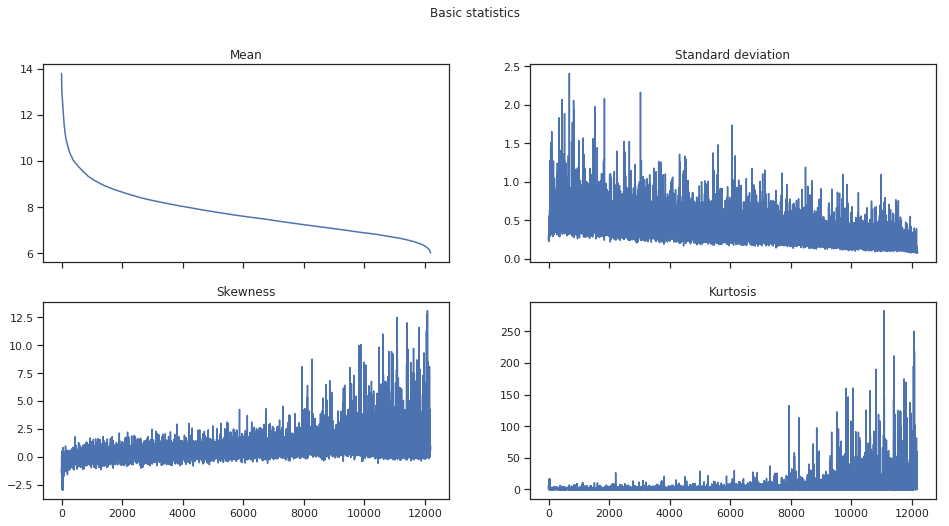
\includegraphics[width=\textwidth]{images/basic_stats.png}
\caption{Main statistical characteristics of the data}
\label{fig:stats}
\end{figure}

On the figure \ref{fig:stats} we can see that the data is not standardized. The variables are sorted decreasingly by means varying from $6.01$ to $13.79$. Also standard deviations vary from $0.07$ to $2.41$. Therefore, before applying any dimensionality reduction method we should standardize our data, e.g in PCA the variance explained by a variable hugely depends on its scale and could lack of standardization could lead to over or underestimation of its effect. Skewness and kurtosis evidence against our normality assumption. They vary from $-2.99$ to $13.10$ and $-1.38$ to $282.88$ respectively. Especially, the kurtosis implies presence of outliers. In order to get more insight on the distribution of our variables in figure \ref{fig:hists_out} we plot the histogram and boxplots of genes with maximum skewness and kurtosis and in figure \ref{fig:hists_norm} we plot histograms and boxplots of randomly chosen genes from the data. 

\begin{figure}
\centering
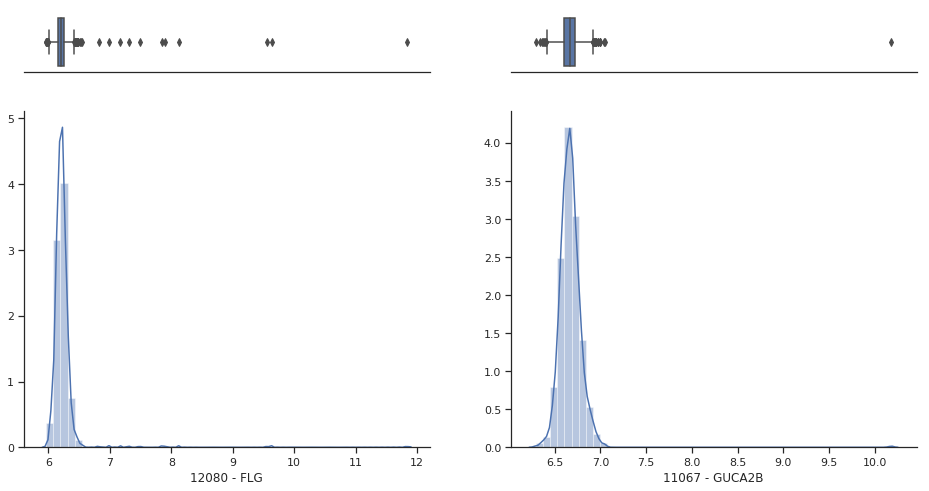
\includegraphics[width=\textwidth]{images/hists_ouliers.png}
\caption{Histograms of genes with maximum skewness and kurtosis}
\label{fig:hists_out}
\end{figure}

\begin{figure}
\centering
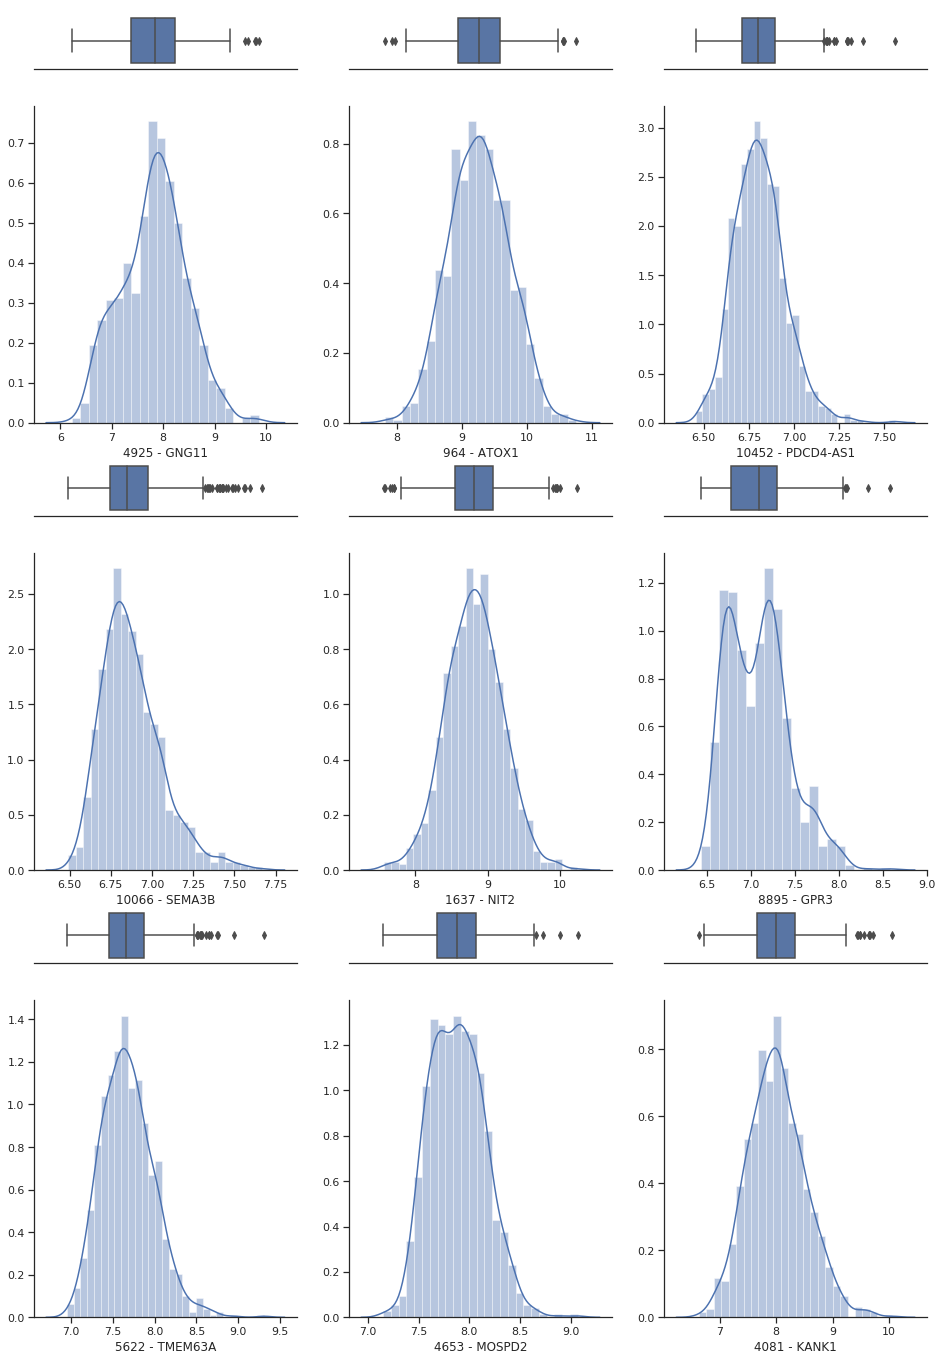
\includegraphics[width=\textwidth]{images/hists_normal.png}
\caption{Histograms of randomly chosen genes from the data}
\label{fig:hists_norm}
\end{figure}


By looking at the figure \ref{fig:hists_norm} we conclude that also the distribution are visibly skewed and even multimodal they do not indicate that further transformation is needed to able to use models assuming normality. However, we can clearly see form figure \ref{fig:hists_out} that high skewness or kurtosis can be caused by outlying values for this variable. In order to verify this we calculate the 95\% quantile for both skewness and kurtosis. They are equal to $2.15$ and $9.77$ respectively. It indicates that only very few genes have statistics indicating strong non normality. What is more, the number of genes with kurtosis or skewness above 95\% quantile is $710$ which is not significantly larger than the number of genes with high kurtosis only. This indicates that the extreme values of either of these statistics appear on the small subset of genes. In order to assess the influence of such genes we consider following data sets: data set consisting of genes only with values of skewness and kurtosis below the 95\% quantile ($D_1$), the complement of the previous data set ($D_2$), $50$ data sets extracted by randomly choosing $710$ variables from the original data ($D_{random}$). We split each of them to train and test parts and fit logistic regression with L1 penalty and regularization hyperparameter chosen using cross validation as described in section \ref{section:selection}. We compare the scores on the test set to check how these genes with outlying values impact our prediction. For the random data sets we fit the model for each of them and take the mean scores. The results are presented in the table \ref{tab:scores-trunc}: 
\begin{table}[H]
\centering
    \begin{tabular}[t]{c c c c c}
    \toprule
    & ROC AUC & Precision & Recall & F1\\
    \midrule
    $D_1$ & $0.827$ & $0.718$ &	$0.712$ & $0.715$ \\
    $D_2$ & $0.742$ & $0.659$ & $0.577$ & $0.615$ \\
    $D_{random}$ & $0.787$ & $0.700$ & $0.616$ & $0.655$ \\
    \bottomrule
\end{tabular}
    \caption{Scores of logistic regression with subsets of variables}
    \label{tab:scores-trunc}
\end{table}

From this table we can clearly see that the genes in $D_2$ do not have big predictive power. The mean scores from $D_{random}$ are higher for every considered metric. It is also worth noting that randomly chosen variables bring less information for prediction than all the genes in $D_1$. The next step is checking how these genes with extreme values impact stability of our classifier.

In order to check it we use six different transformations on the data, then fit logistic regression model with L1 penalty and the same regularization parameter. We choose this classifier because its weights are sensitive to outliers and could easily indicate the impact of genes with extreme values. 
The compared transformations are:

\begin{enumerate}
    \item No transformation
    \item Standardization - from each variable we subtract its mean and divide by standard deviation
    \item Quantile transformation to normal distribution - for each variable we calculate the empirical cumulative density function (CDF) and use it to project original data. The projected data is truncated to $10^{-7}$ and $1-10^{-7}$ then transformed using inverse CDF of normal distribution. The formula is $y_{i}=\Phi^{-1}\left(F\left(x_{i}\right)\right),$ where $F$ and $\Phi$ represent empirical CDF and normal distribution CDF respectively. This transformation is more robust to outliers than scaling but may deform distances within and across features.
    \item Quantile transformation to uniform distribution - similar to the previous one but we transform data to match uniform distribution. We use it to check how the weights of logistic regression will be affected when unreasonable transformation is applied to our data.
    \item Truncating most extreme values - for each feature we calculate 1\% ($q_1$) and 99\% ($q_{99}$) quantiles and replace values smaller then $q_1$ with $q_1$ and values greater then $q_{99}$ with $q_{99}$
    \item Quartile standardization - for each variable we subtract its median and divide by inter quartile range which is equal to difference between 75\% quantile and 25\% quantile
\end{enumerate}

\begin{figure}
\centering
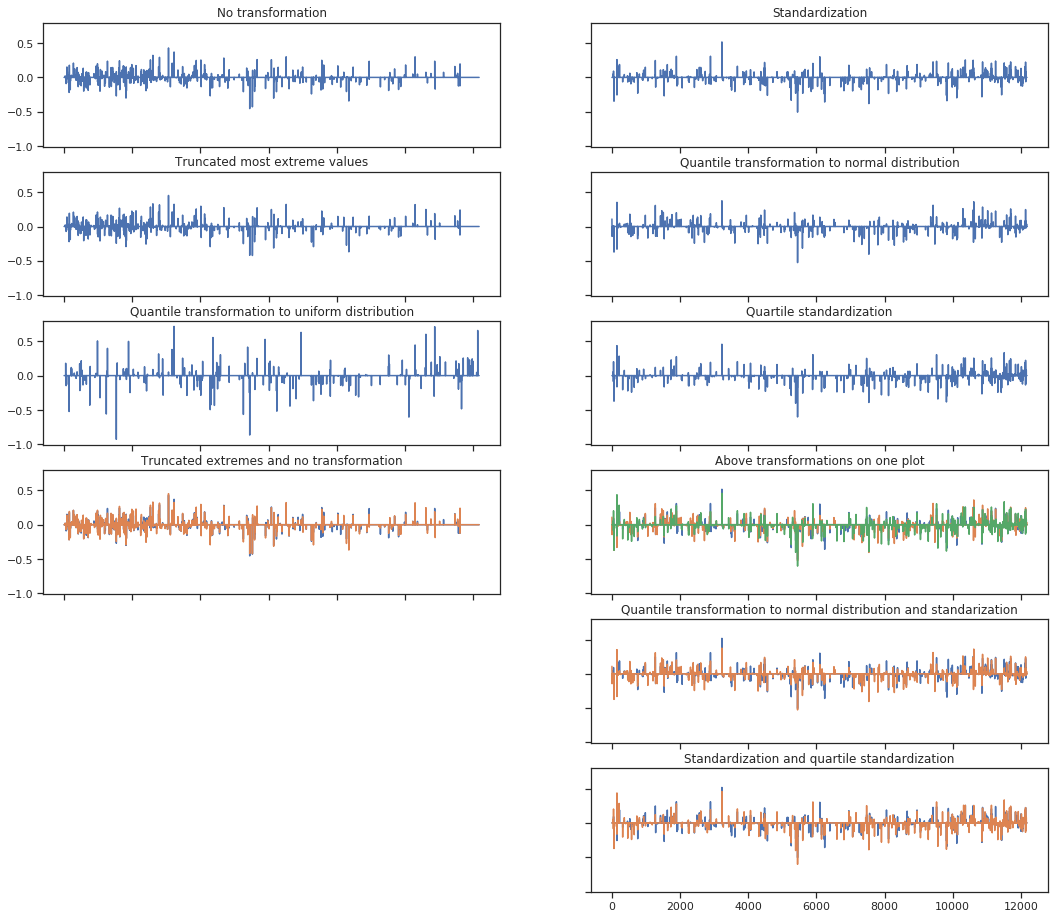
\includegraphics[width=\textwidth]{images/normalization_coeffs.png}
\caption{Weights of logistic regression with different data transformations}
\label{fig:normalization}
\end{figure}

The plots of the weights of these classifiers are presented on figure \ref{fig:normalization}. We can see that the difference between no transformation and truncating extreme values ($4$-th plot in the first column) is very small. It indicates that these genes with very high skewness and kurtosis do not impact our prediction significantly and do not need to be truncated or removed from the data. What is more application of different transformation aiming to normalize our features (plots $4-6$-th in the second column) resulted in similar logistic regression coefficients. Taking into account figure \ref{fig:hists_norm} and \ref{fig:normalization} we conclude that there is no justification of using other transformation of our data set before further analysis. We will only standardize the data before applying dimensionality reduction methods as they are sensitive to features' scales.

In data mining we usually aim to remove strongly correlated variables from the data, due to the possibility of causing instability in our models (\cite{Correlation}). In case of gene expression data this usually refers to genes which are co-regulated and involved in the same genetic pathway. In order to get notion of such correlation structure we present (figure \ref{fig:heatmap}) the correlation between randomly chosen $50$ genes. 

Although most variables seem to have correlation close to $0$ we can clearly see some significant ones, even though we chosen randomly only $0.41$\% of our variables. We may also look at the histogram of correlations of features with response (figure \ref{fig:corrHist}). We can see that majority of variables has low correlation coefficient indicating that the dependencies between the response and other variables are hidden and rather complex. These two figures strongly indicate that dimensionality reduction methods (both feature selection and extraction) can be exploited on our data.

\begin{figure}
\centering
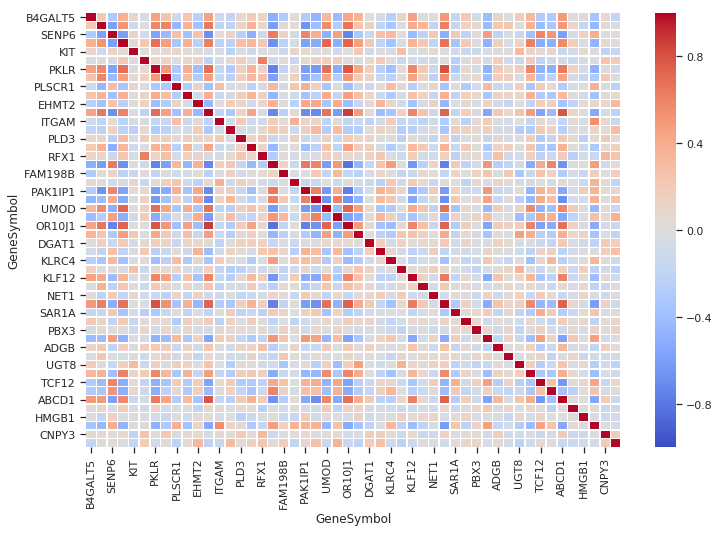
\includegraphics[width=\textwidth]{images/heatmap.png}
\caption{Correlation of randomly chosen subset of $50$ genes}
\label{fig:heatmap}
\end{figure}

\begin{figure}
\centering
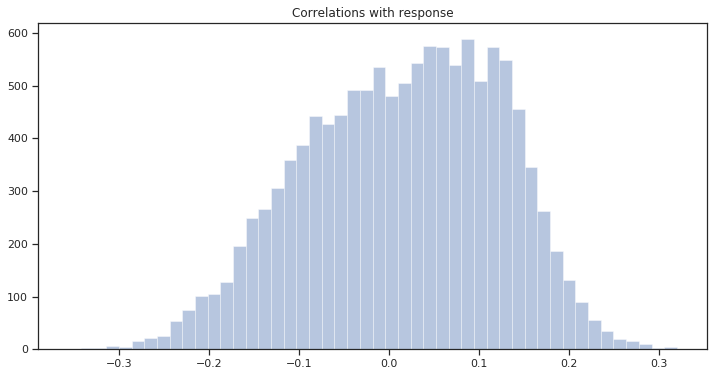
\includegraphics[width=\textwidth]{images/corrHist.png}
\caption{Histogram of correlations of features with response}
\label{fig:corrHist}
\end{figure}

\chapter{Results} \label{section:results}

Reduction and selection should be performed within cross validation

\begin{itemize}
    \item Something about code - used libraries, computational power, implementations etc.
    \item Best models - present ROC curves, adjust errors from ROC, some explanation, comparison with model chosen by recall
    \item comparison with other papers - e.g. most popular classification based on 76 selected genes
\end{itemize}


\chapter{Applications in medicine} \label{section:application}

\begin{itemize}
    \item What is acceptable in medicine
    \item Not liking black box models, Linear vs nonlinear
    \item Feature extraction vs feature selection
    \item pathway enrichment
\end{itemize}

\chapter{Conclusion} \label{section:summary}

\bibliography{biblio}
\bibliographystyle{plain}
%\bibliographystyle{apalike}


\end{document}
